\chapter{Especificación del Sistema}
\label{cap:especificacion_sistema}

\section{Visión General de la Arquitectura}

El sistema se articula en torno a tres componentes desacoplados que se comunican a través de interfaces de red local:

\begin{enumerate}
    \item \textbf{El Servidor de Orquestación (Node.js 24 + Python 3.12, Ubuntu Server 24.04 LTS):} Ejecutado en la torre Ryzen (APU, 16 GB RAM) en modo \textit{headless}, alberga el núcleo lógico del ecosistema. El \textit{gateway} de OpenClaw~\cite{openclaw} (Node.js 24) actúa como orquestador principal, proporcionando los canales de usuario (Telegram, \textit{dashboard} web) y la interfaz de agentes de IA. Los \textit{drivers} de dispositivos (Python) son invocados mediante \texttt{exec} desde las \textit{tools} del orquestador. La administración se realiza mediante Cockpit (puerto 9090) y SSH con llaves RSA.
    \item \textbf{El Entorno de Desarrollo (Portátil):} Conserva las herramientas de ingeniería, como Arduino CLI para compilación de firmware ESP32, \LaTeX{} para la redacción de la memoria y Git para control de versiones, y se conecta al servidor exclusivamente mediante SSH. Esta separación garantiza que las tareas de desarrollo (compilaciones, pruebas, reinicios) no interfieran con el bucle de control domótico en producción.
    \item \textbf{El Nodo Firmware (C++20):} Ejecutado en el ESP32 DevKit V1~\cite{espressif_esp32_trm}, actúa como un puente hardware especializado que traduce comandos de red a tramas del bus LIN~\cite{iso_17987_2025} propietario de la máquina HVAC. \textbf{[Pendiente de implementar.]}
\end{enumerate}

La comunicación entre todos los componentes se produce exclusivamente sobre la red \textit{air-gapped} (\texttt{192.168.1.0/24}), garantizando que ningún dato de telemetría abandone el perímetro local.

\begin{figure}[h]
\centering
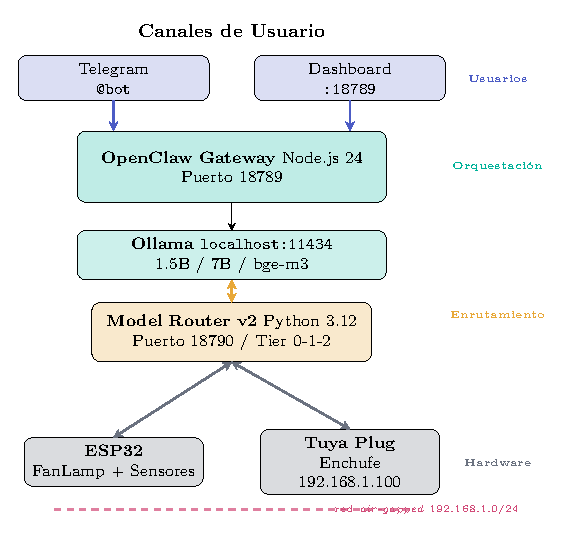
\includegraphics[width=\textwidth]{img/fig_8_1.pdf}
\caption{Arquitectura de tres capas del ecosistema Luxe Core AI. Las flechas indican flujo de comunicación entre componentes.}
\label{fig:arquitectura}
\end{figure}


\section{Topología de Red Local}

El ecosistema opera sobre un segmento de red físicamente aislado de Internet, implementado mediante un router \textbf{TP-Link TL-MR6400} que actúa exclusivamente como \textit{switch} Ethernet y punto de acceso WLAN. Este dispositivo (cedido temporalmente y con la ranura SIM rota a nivel \textit{hardware}) carece de cualquier tipo de enlace WAN, lo que garantiza que ningún paquete pueda abandonar el segmento local sin intervención explícita del administrador.

\begin{figure}[h]
\centering
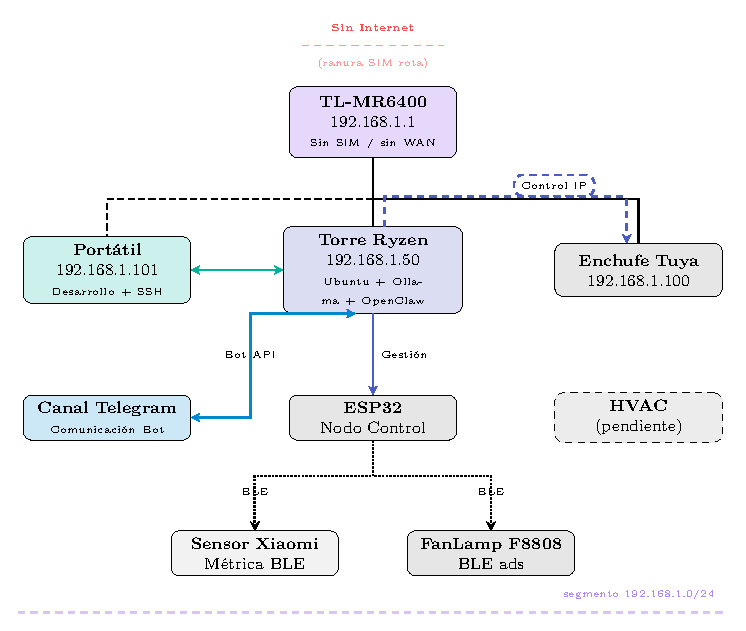
\includegraphics[width=\textwidth]{img/fig_8_2.pdf}
\caption{Topología de despliegue del ecosistema sobre la red air-gapped. Las líneas continuas indican Ethernet, las discontinuas Wi-Fi, y las punteadas BLE. El control del ventilador y el sensor se realiza a través del ESP32 como puente BLE, mientras que el enchufe Tuya se comunica directamente por IP local.}
\label{fig:despliegue}
\end{figure}

\subsection{Asignación de Direcciones IP}

Todas las direcciones del segmento se asignan de forma estática para garantizar la previsibilidad de las comunicaciones y eliminar la dependencia de un servidor DHCP:

\begin{table}[h]
\centering
\begin{tabular}{|l|l|l|p{4cm}|}
\hline
\textbf{Dispositivo} & \textbf{IP} & \textbf{Interfaz} & \textbf{Función} \\
\hline
Servidor (Torre Ryzen) & \texttt{192.168.1.50/24} & Ethernet (\texttt{enp3s0}) & Orquestador OpenClaw + Ollama \\
Portátil de desarrollo & \texttt{192.168.1.101/24} & Wi-Fi (\texttt{wlp45s0}) & Desarrollo y administración \\
Router TP-Link TL-MR6400 & \texttt{192.168.1.1/24} & Interna & \textit{Switch} + AP WLAN \\
Enchufe Tuya & \texttt{192.168.1.100/24} & Wi-Fi & Actuador del extractor \\
\hline
\end{tabular}
\caption{Asignación estática de direcciones IP en el segmento air-gapped.}
\end{table}

\subsection{Ventana de Conectividad de Contingencia}

Para situaciones que requieran acceso puntual a Internet, como la instalación inicial, actualizaciones de seguridad o la descarga de nuevos modelos de lenguaje, se ha documentado un procedimiento de \textbf{pasarela de contingencia} mediante el cual el portátil de desarrollo actúa como enrutador NAT entre el segmento \textit{air-gapped} y una conexión celular externa. Este procedimiento está detallado en el Capítulo~5 y está diseñado para ser estrictamente temporal.

\subsection{Topología Física}

El router TL-MR6400 proporciona cuatro puertos Ethernet LAN y conectividad WLAN 802.11n en la banda de 2.4~GHz. La conexión del servidor se realiza mediante un cable Ethernet directo a uno de los puertos \textbf{LAN dedicados} del router (no al puerto híbrido LAN/WAN), para evitar el problema de aislamiento eléctrico documentado en el Capítulo~5.

\section{Decisiones de Diseño}
\label{sec:decisiones_diseno}

A lo largo del proyecto se tomaron decisiones arquitectónicas y técnicas que fueron registradas formalmente como \textit{Architecture Decision Records} (ADR). La Tabla~\ref{tab:adrs} resume las nueve decisiones documentadas, indicando dónde se discute cada una en esta memoria y su estado actual.

\begin{table}[h]
\centering
\begin{tabular}{|p{0.6cm}|p{3.8cm}|p{3cm}|p{4.5cm}|}
\hline
\textbf{ADR} & \textbf{Título} & \textbf{Referencia en la memoria} & \textbf{Estado} \\
\hline
001 & Entorno híbrido UCO (Conda + uv) & Cap.~4 y Cap.~5 & Superado por ADR-001b \\
001b & Migración a arquitectura Edge local & Cap.~5 (sección 5.3) & Implementado \\
002 & Aislamiento de red y Hotspot Spoofing & Cap.~5 (sección 5.5) & Implementado \\
003 & Lectura GATT directa de sensores Xiaomi & Cap.~5 (sección 5.5.2) y Cap.~8 & Implementado \\
004 & Validación Tuya en red air-gapped & Cap.~8 (sección Tuya) & Implementado \\
005 & Protocolo FanLamp por anuncios BLE & Cap.~8 (sección FanLamp) & Implementado \\
006 & Infraestructura de servidor y Ubuntu Server 24.04 & Cap.~5 (sección 5.6) & Implementado \\
007 & Despliegue de red y contingencia NAT & Cap.~5 (sección 5.7) & Documentado \\
008 & Migración de CMDOP a OpenClaw npm & Cap.~4 (sección 4.3) y Cap.~8 & Implementado \\
\hline
\end{tabular}
\caption{Architecture Decision Records (ADR) del proyecto, con referencias a los capítulos donde se detalla cada decisión.}
\label{tab:adrs}
\end{table}

Los documentos completos de cada ADR están disponibles en el repositorio del proyecto, en el directorio \texttt{docs/design\_decisions/}.

\section{Módulos del Servidor}

\subsection{Orquestador OpenClaw (Node.js)}

El \textit{gateway} de OpenClaw~\cite{openclaw} se ejecuta sobre \textbf{Node.js 24} como un servicio \texttt{systemd --user} en el puerto~18789, accesible desde toda la subred \texttt{192.168.1.0/24}. Proporciona de forma nativa:

\begin{itemize}
    \item \textbf{Canal Telegram:} integración directa con la API de BotFather, sin necesidad de scripts Python auxiliares.
    \item \textbf{\textit{Dashboard} web:} interfaz de administración accesible en \texttt{http://192.168.1.50:18789}.
    \item \textbf{Búsqueda web:} integración con Gemini API para consultas externas bajo demanda. Requiere conexión a Internet a través de la pasarela de contingencia (Capítulo~\ref{cap:restricciones_metodologia}); es una funcionalidad opcional que no afecta al control local de los dispositivos.
    \item \textbf{Ejecución de herramientas (\textit{exec}):} invocación de los \textit{drivers} Python de dispositivos mediante \texttt{server/tools/}.
\end{itemize}

El motor de inferencia se apoya en \textbf{Ollama} (\texttt{localhost:11434}) con los modelos \texttt{qwen2.5-coder:1.5b} (clasificador, siempre en RAM) y \texttt{qwen2.5-coder:7b-instruct} (razonador, bajo demanda), más \texttt{bge-m3}~\cite{bge_m3} para \textit{embeddings} semánticos. Toda la comunicación se mantiene dentro del segmento \textit{air-gapped}.

\subsection{Arquitectura de Enrutamiento Inteligente (Model Router v2)}
\label{sec:model_router_v2}

\begin{figure}[h]
\centering
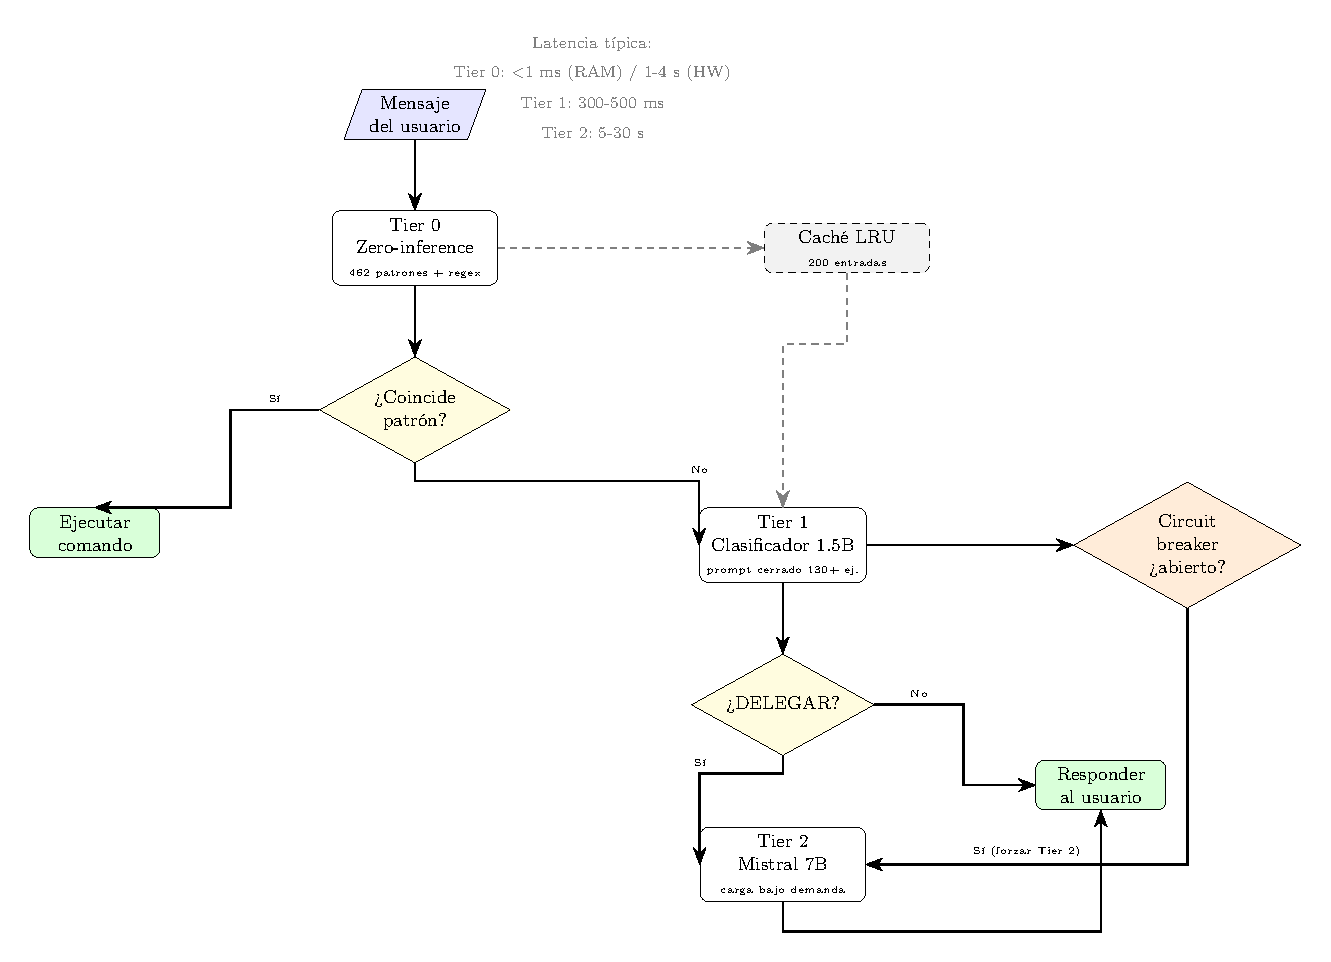
\includegraphics[width=\textwidth]{img/fig_8_3.pdf}
\caption{Flujo de enrutamiento del Model Router v2. El mensaje pasa por tres niveles de complejidad creciente, con un circuit breaker que deriva al Tier 2 si el clasificador 1.5B no está disponible.}
\label{fig:router_flow}
\end{figure}

El Model Router v2 implementa un servidor HTTP (Python 3.12, puerto~18790) con una API compatible con OpenAI que enruta cada mensaje del usuario a través de tres niveles de complejidad creciente. La decisión de usar tres niveles, y no dos, se tomó después de probar una configuración inicial con un modelo 14B como razonador pesado y un 7B como ligero. El rendimiento en el hardware disponible (Ryzen 5, 16~GB RAM) resultó insuficiente: el 14B introducía latencias de más de un minuto en consultas simples. Se reconfiguró entonces como 1.5B (clasificador ligero) + 7B (razonador), manteniendo \texttt{bge-m3} para \textit{embeddings} semánticos, elegido desde el inicio por su eficiencia en RAM y su capacidad multilingüe (español e inglés).

\begin{enumerate}
    \item \textbf{Tier 0 --- Zero-inference:} Realiza \textit{pattern matching} directo sin necesidad de modelos de lenguaje. Su primera versión incluía 127 patrones exactos y expresiones regulares, capturando aproximadamente el 80\% de los comandos diarios. Tras sucesivas ampliaciones, el sistema alcanzó los 462 patrones, elevando la cobertura a aproximadamente el 92\% con una latencia inferior a 1~ms para consultas de estado en RAM y entre 1,5 y 4~s para comandos de hardware (limitado por el ESP32).
    \item \textbf{Tier 1 --- Clasificador 1.5B:} Utiliza el modelo \texttt{qwen2.5-coder:1.5b} con un \textit{prompt} cerrado de más de 130 ejemplos categorizados (iluminación, ventilador, escenas, consultas, delegación). El modelo responde exclusivamente con JSON estructurado o el token \texttt{DELEGAR}. Parámetros optimizados: \texttt{num\_ctx=2048}, \texttt{max\_tokens=256}, \texttt{temperature=0.0}. Latencia típica: 300--500~ms en Ryzen 5.
    \item \textbf{Tier 2 --- Razonador 7B:} Emplea el modelo \texttt{qwen2.5-coder:7b-instruct}, que se carga bajo demanda con \texttt{keep\_alive=0} y se descarga automáticamente tras 5 minutos de inactividad. Gestiona conversaciones abiertas, análisis y resolución de problemas, con una latencia de 5--30~s.
\end{enumerate}

Además de los niveles de enrutamiento, el Model Router v2 incorpora:

\begin{itemize}
    \item \textbf{Caché de comandos (LRU, 200 entradas):} Evita reclasificar mensajes repetidos, reduciendo la carga del modelo 1.5B en aproximadamente un 15\% adicional.
    \item \textbf{DeviceStateManager:} Repositorio del estado de cada dispositivo (luz, ventilador, enchufe, sensor) mantenido en RAM con acceso \textit{thread-safe}. Permite responder consultas como ``cómo está la casa'' en menos de 1~ms sin necesidad de interactuar con el hardware.
    \item \textbf{Precomputación de \textit{embeddings}:} Clasificación semántica mediante \texttt{bge-m3} con \textit{embeddings} precalculados al arranque (15 intenciones) y similitud coseno. Se utiliza como \textit{fallback} del Tier 1 cuando el \textit{keyword matching} no encuentra correspondencia.
\end{itemize}

\subsection{Auto-Recuperación y Tolerancia a Fallos}
\label{sec:auto_recuperacion}

El sistema incorpora mecanismos para garantizar su robustez y disponibilidad, minimizando el impacto de fallos tanto en los subsistemas de inferencia como en los dispositivos de hardware:

\begin{itemize}
    \item \textbf{Circuit Breaker para modelos:} Patrón \textit{circuit breaker} con tres estados (CLOSED, OPEN, HALF\_OPEN) para los subsistemas de Ollama (modelos 1.5B y 7B). Si un modelo falla 3 veces consecutivas, el circuito se abre durante 30~segundos, evitando reintentos inútiles. La recuperación es automática mediante sondeo en estado HALF\_OPEN.
    \item \textbf{Reintentos con \textit{backoff} exponencial para hardware:} Los comandos ejecutados a través de \texttt{home.sh} reintentan hasta 2 veces con \textit{backoff} exponencial (1~s, 3~s) y un \textit{jitter} aleatorio. Se distinguen errores transitorios (\textit{timeout}, puerto serie ocupado, dispositivo desconectado) de errores permanentes (validación, permisos).
    \item \textbf{Auto-reset de puerto USB:} Ante un error de puerto serie (\texttt{SerialException}), el sistema intenta reiniciar el dispositivo USB del ESP32 mediante las operaciones de \textit{unbind/rebind} en \texttt{/sys/bus/usb/drivers/usb/}.
    \item \textbf{SelfHealManager:} Un hilo demonio verifica cada 30~segundos la salud de Ollama (recargando modelos caídos), la conectividad del ESP32 (\texttt{/dev/ttyUSB0}) y el estado de los \textit{circuit breakers}. Su operación es totalmente autónoma.
    \item \textbf{Health check proactivo ESP32:} Antes de ejecutar cualquier comando del ventilador, se verifica la existencia de \texttt{/dev/ttyUSB0}. Si el puente está desconectado, se notifica al usuario de inmediato.
    \item \textbf{Mensajes de recuperación visibles:} Cuando un reintento tiene éxito, el usuario recibe un mensaje con el prefijo \texttt{[RECUPERADO tras N reintento(s)]}, proporcionando transparencia sobre la resiliencia del sistema.
\end{itemize}

\subsection{Daemon de Sensorización Continua}
\label{sec:sensor_daemon}

El \textbf{Sensor Daemon} (\texttt{sensor\_daemon.py}) es un servicio \texttt{systemd} que lee el sensor BLE Xiaomi LYWSD03MMC cada 60~segundos a través del puente ESP32. Almacena dos salidas:

\begin{itemize}
    \item \texttt{/tmp/latest\_sensor.json} --- Última lectura (temperatura, humedad, batería, RSSI, \textit{timestamp} UTC). Lectura atómica (\textit{write} + \textit{rename}) para evitar lecturas parciales.
    \item \texttt{/tmp/sensor\_history.jsonl} --- Histórico completo en formato JSON Lines, con rotación automática a 50.000 líneas (~5~MB).
\end{itemize}

La integración con el router de modelos reduce la latencia de las consultas de temperatura de 18~s (escaneo BLE síncrono) a 0--1~ms, leyendo directamente de \texttt{latest\_sensor.json}. Adicionalmente, si hay conexión a Internet disponible mediante la pasarela de contingencia (Capítulo~\ref{cap:restricciones_metodologia}), cada lectura puede incluir condiciones meteorológicas exteriores de \texttt{wttr.in} con una caché de 10~minutos para no saturar la API gratuita.

\subsection{Asesor de Confort Térmico (Comfort Advisor)}
\label{sec:comfort_advisor}

\begin{figure}[h]
\centering
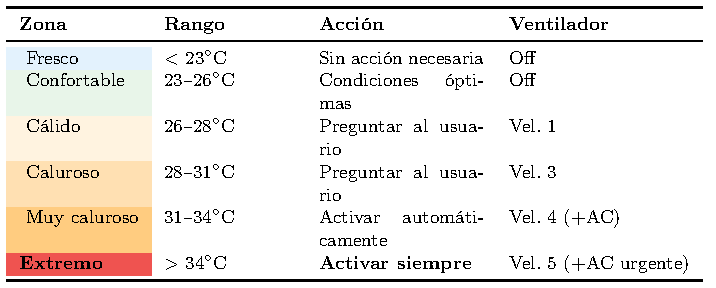
\includegraphics[width=0.85\textwidth]{img/fig_8_4.pdf}
\caption{Zonas de confort térmico adaptadas al clima andaluz. Las zonas se asignan en función del índice de calor NOAA, combinando temperatura y humedad relativa.}
\label{fig:zonas_confort}
\end{figure}

El \textbf{Comfort Advisor} (\texttt{server/model\_router/comfort.py}) evalúa el confort térmico de la habitación siguiendo los criterios del estándar ASHRAE 55~\cite{ashrae55_2023}, basándose en las lecturas de temperatura y humedad del sensor:

\begin{itemize}
    \item \textbf{Índice de calor (Heat Index) NOAA:} Implementación de la fórmula de Rothfusz~\cite{rothfusz_1990} para calcular la sensación térmica a partir de temperatura y humedad relativa, con conversión explícita $^\circ$C $\leftrightarrow$ $^\circ$F.
    \item \textbf{Zonas de confort adaptadas al clima andaluz:} 6 niveles progresivos:
    \begin{enumerate}
        \item Fresco ($<$ 23$^\circ$C) --- sin acción necesaria.
        \item Confortable (23--26$^\circ$C) --- condiciones óptimas.
        \item Cálido (26--28$^\circ$C) --- ventilador a velocidad 1.
        \item Caluroso (28--31$^\circ$C) --- ventilador a velocidad 3.
        \item Muy caluroso (31--34$^\circ$C) --- ventilador a velocidad 4 y considerar AC.
        \item Extremo ($>$ 34$^\circ$C) --- ventilador a velocidad 5 y AC urgente.
    \end{enumerate}
    \item \textbf{Evaluación de humedad:} Tres estados (seco, < 35\% HR; óptimo, 35--70\%; húmedo, > 70\%) con recomendaciones específicas.
    \item \textbf{Detección de tendencia:} Comparación de la temperatura actual con lecturas de los últimos 30~minutos para determinar si la temperatura sube, baja o se mantiene estable, expresado en $^\circ$C/hora.
\end{itemize}

\subsection{Asesor Inteligente con Contexto Exterior (Smart Advisor)}
\label{sec:smart_advisor}

El \textbf{Smart Advisor} (\texttt{server/model\_router/smart\_advisor.py}) amplía el Comfort Advisor incorporando datos del entorno exterior y el estado de presencia del usuario:

\begin{itemize}
    \item \textbf{Comparación interior vs.\ exterior:} Contrasta temperatura y humedad interiores (sensor BLE) con las exteriores (vía \texttt{wttr.in}, si hay conexión a Internet) y emite recomendaciones contextuales.
    
    \item \textbf{Lógica de ventana y persiana:} Algoritmo de decisión que recomienda abrir o cerrar ventanas y bajar persianas basándose en la diferencia térmica (umbral: 2$^\circ$C), el índice UV exterior (umbral: 5), la temperatura máxima para ventilar (32$^\circ$C) y la detección de lluvia.
    
    \item \textbf{Detección de presencia:} Sistema híbrido con tres métodos complementarios:
    \begin{enumerate}
        \item \textbf{Manual:} Los comandos ``me voy'' y ``he llegado'' (~15 variantes) actualizan un \textit{flag} en \texttt{/tmp/luxe\_presence.json}. Timeout de 30~minutos.
        \item \textbf{BLE:} Escaneo del teléfono móvil mediante \texttt{bluetoothctl scan le}, buscando una dirección MAC configurable.
        \item \textbf{Por IP en Wi-Fi:} Cuando el teléfono del usuario se conecta a la red Wi-Fi local, se asigna una IP estática conocida. El sistema puede detectar presencia verificando si esa IP responde en la subred \texttt{192.168.1.0/24}, sin necesidad de escaneo BLE. Este método es más rápido (un \texttt{ping} de 1--2~ms) y no depende del hardware Bluetooth del servidor. \textbf{[Pendiente de implementar.]}
    \end{enumerate}
    
    \item \textbf{Filosofía \textit{Human in the Loop}:} El sistema está diseñado para \textbf{preguntar antes de actuar} siempre que sea razonable. Las auto-acciones solo se ejecutan sin consultar cuando hay certeza de que el usuario se beneficiará (zona extrema, dos o más saltos de nivel térmico). En cualquier otra situación, el sistema pregunta y espera confirmación. Esta filosofía evita la sensación de pérdida de control que muchos sistemas autónomos generan en los usuarios, y refuerza la confianza en el ecosistema. La regla es simple: el sistema sugiere, el usuario decide.
    
    \item \textbf{Auto-acciones condicionales:} El daemon evalúa tras cada lectura si debe actuar según reglas de cambio de zona térmica:
    \begin{itemize}
        \item Misma zona $\rightarrow$ no actuar (evitar molestias).
        \item +1 zona $\rightarrow$ preguntar al usuario.
        \item +2 o más zonas $\rightarrow$ actuar automáticamente (prioridad de confort).
        \item Zona Extrema $\rightarrow$ actuar siempre.
        \item Sin presencia $\rightarrow$ nunca actuar (ahorro energético).
        \item Excepción: si el usuario subió manualmente el ventilador y la zona empeora, se incrementa automáticamente la velocidad, respetando su intención.
    \end{itemize}
\end{itemize}

\subsection{Comunicación y Notificaciones}
\label{sec:comunicacion_notificaciones}

\begin{itemize}
    \item \textbf{462+ comandos en lenguaje natural:} El Tier~0 reconoce más de 462 patrones en español coloquial, incluyendo variantes con muletillas, dialectalismos andaluces y formas abreviadas. Cobertura completa de iluminación (35 variantes), ventilador (50 variantes), escenas (40 variantes) y consultas (15 variantes).
    
    \item \textbf{8 escenas predefinidas:} noche, apagar todo, encender todo, relax, cine, lectura, fiesta y estudio. Cada escena ejecuta una secuencia de comandos hardware.
    
    \item \textbf{Notificaciones proactivas vía Telegram:} Una tarea programada (cada 2~minutos) reenvía las notificaciones del Smart Advisor al canal de Telegram, incluyendo acciones ejecutadas y preguntas pendientes de confirmación.
    
    \item \textbf{API compatible con OpenAI:} El router expone \texttt{/v1/chat/completions}, permitiendo a cualquier cliente compatible consumir el servicio de enrutamiento sin modificar el código.
\end{itemize}

\subsection{Infraestructura de Despliegue}
\label{sec:infraestructura_despliegue}

\begin{itemize}
    \item \textbf{Tres servicios \texttt{systemd} persistentes:}
    \begin{itemize}
        \item \texttt{model-router.service} --- enrutador 3 niveles (Python 3.12, puerto~18790).
        \item \texttt{sensor-daemon.service} --- lectura continua del sensor (cada 60~s).
        \item \texttt{openclaw-gateway.service} --- orquestador principal (Node.js 24, puerto~18789).
    \end{itemize}
    Todos con auto-arranque y reinicio automático ante fallos (\texttt{Restart=always}).
    
    \item \textbf{Endpoint de monitorización:} \texttt{GET /status} devuelve métricas en tiempo real: estado de los modelos en Ollama, salud del ESP32, circuit breakers, estadísticas de caché, estado de dispositivos y \textit{uptime}.
    
    \item \textbf{Robustez del puente ESP32:} El script \texttt{fanlamp\_control.py} incorpora reintentos internos (3 intentos), manejo seguro del puerto serie y \textit{timeouts} configurables.
\end{itemize}

\subsection{Métricas de Rendimiento}
\label{sec:metricas_rendimiento}

La Tabla~\ref{tab:latencia_antes_despues} resume la mejora de latencia conseguida tras la implementación del Model Router v2 y el Sensor Daemon. Las mediciones se realizaron sobre el hardware real del servidor (Ryzen 5, 16~GB RAM) con el ESP32 conectado por USB.

\begin{table}[h]
\centering
\begin{tabular}{|l|c|c|c|}
\hline
\textbf{Escenario} & \textbf{Latencia antes} & \textbf{Latencia ahora} & \textbf{Modelo usado} \\
\hline
``velocidad 3'' & $\sim$2 s & $\sim$1,5 s (hardware) & Ninguno (Tier 0) \\
``cómo está la casa'' & $\sim$2 s & 0--1 ms (RAM) & Ninguno (Tier 0) \\
``me puedes encender la luz'' & $\sim$3 s & $\sim$300 ms & 1.5B clasificador \\
``buenos días'' & $\sim$12 s (2 modelos) & 5--30 s (directo 7B) & Solo 7B (Tier 2) \\
``temperatura'' & 18 s (BLE scan) & 0--1 ms (daemon) & Ninguno (Tier 0) \\
``qué temperatura hay fuera'' & --- (no existía) & 0--1 ms (caché wttr.in) & Ninguno (Tier 0) \\
\hline
\end{tabular}
\caption{Mejora de latencia tras la implementación del Model Router v2 y el Sensor Daemon.}
\label{tab:latencia_antes_despues}
\end{table}

\subsection{Canales de Usuario}

La interacción con el usuario se realiza a través de dos canales nativos del \textit{gateway} de OpenClaw:

\begin{itemize}
    \item \textbf{Telegram:} Integración nativa con la API de BotFather. Los mensajes se enrutan directamente al agente de IA.
    \item \textbf{\textit{Dashboard} web:} Interfaz accesible en \texttt{http://192.168.1.50:18789} desde cualquier navegador de la subred.
\end{itemize}

La Figura~\ref{fig:telegram} muestra una conversación real con Luxe Core AI a través de Telegram. En ella se aprecia cómo el bot interpreta comandos en lenguaje natural, desde consultas de temperatura hasta control directo del ventilador, sin necesidad de memorizar órdenes concretas. Toda la comunicación se procesa en el servidor local; ningún mensaje abandona la subred.

\begin{figure}[h]
\centering
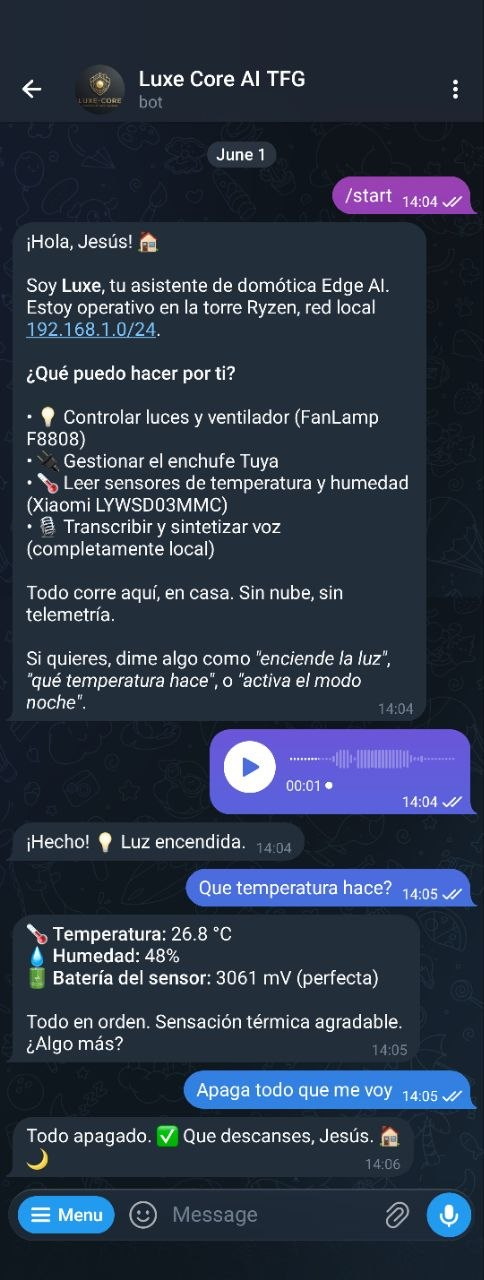
\includegraphics[width=0.5\textwidth]{img/hw_telegram_chat.jpg}
\caption[Interacción por Telegram.]{Interacción con Luxe Core AI a través del canal de Telegram. El bot responde en lenguaje natural a comandos de control, consultas de estado y peticiones conversacionales.}
\label{fig:telegram}
\end{figure}

\begin{figure}[h]
\centering
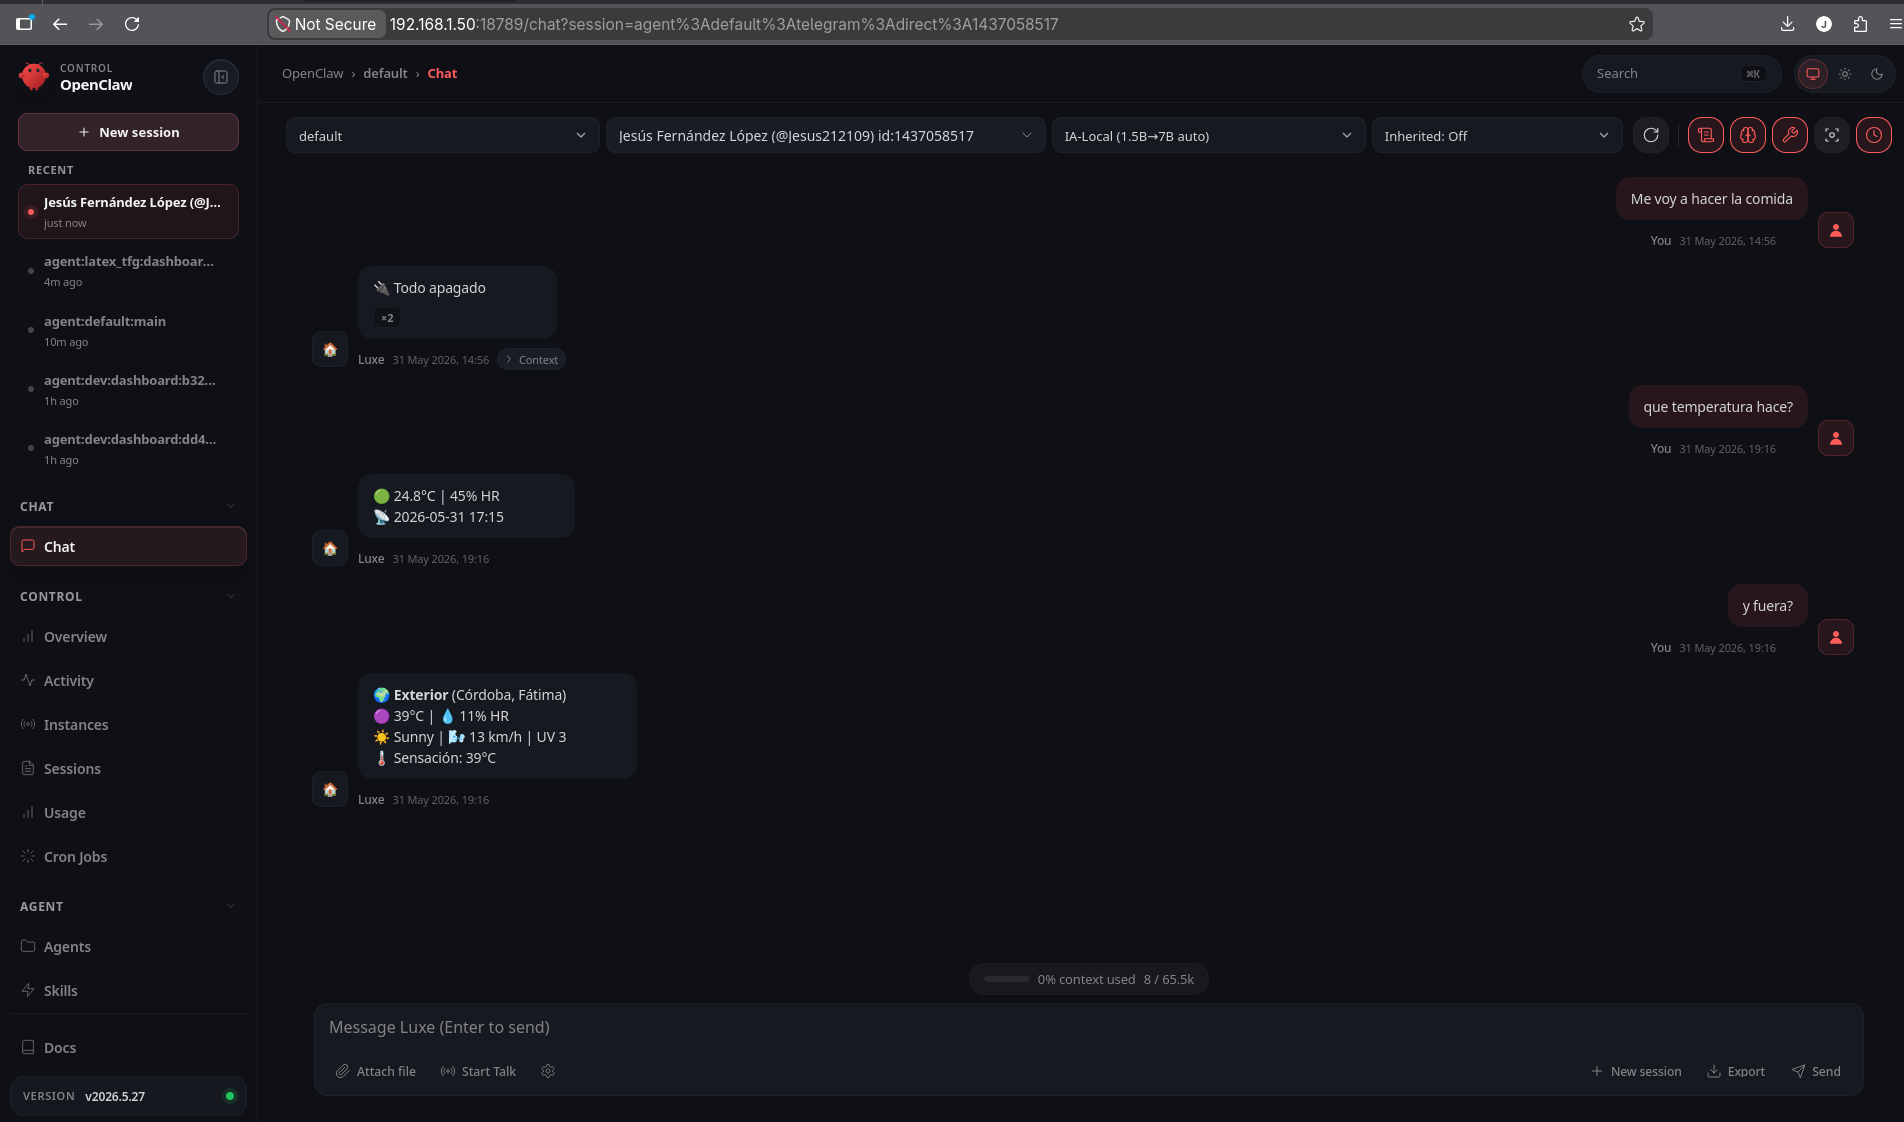
\includegraphics[width=\textwidth]{img/hw_dashboard.png}
\caption[\textit{Dashboard} web de OpenClaw.]{\textit{Dashboard} web del \textit{gateway} de OpenClaw, accesible desde cualquier navegador de la subred local. Desde esta interfaz se pueden consultar los agentes, el estado del sistema y ejecutar comandos de administración.}
\label{fig:dashboard}
\end{figure}

\subsection{Módulo de Integración Tuya}

Este módulo, validado el 13 de mayo de 2026, implementa el control local del enchufe inteligente Tuya mediante \texttt{tinytuya}~\cite{tinytuya} (protocolo 3.5). Los parámetros de conexión se encapsulan en un \textit{dataclass} \texttt{TuyaDeviceConfig} con \texttt{device\_id}, \texttt{local\_key} (almacenada exclusivamente en local), \texttt{address} (\texttt{192.168.1.100}), \texttt{version} (3.5) y \texttt{timeout} (5~s).

La Figura~\ref{fig:tuya_hw} muestra el hardware de esta integración. A la izquierda, el enchufe inteligente Tuya, que fue adquirido en AliExpress por su compatibilidad con el protocolo local 3.5. A la derecha, el humidificador ultrasónico de 24~V que alimenta: un dispositivo originalmente ``tonto'' que, al conectarse al enchufe inteligente, adquiere control remoto y capacidad de programación horaria, integrándose en el ecosistema como un actuador más.

\begin{figure}[h]
\centering
\begin{subfigure}[b]{0.45\textwidth}
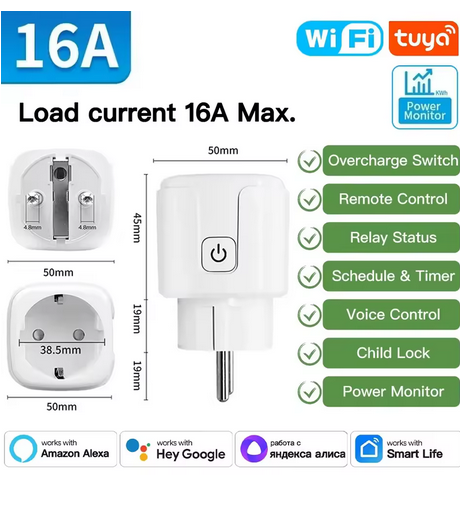
\includegraphics[width=\textwidth]{img/hw_tuya_plug.png}
\caption{Enchufe inteligente Tuya con monitor de consumo.}
\label{fig:tuya_plug}
\end{subfigure}
\hfill
\begin{subfigure}[b]{0.45\textwidth}
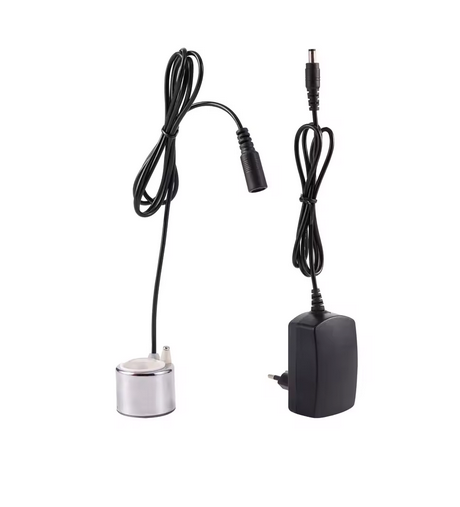
\includegraphics[width=\textwidth]{img/hw_humidifier.png}
\caption{Humidificador ultrasónico de 24V, controlado mediante el enchufe Tuya.}
\label{fig:humidifier}
\end{subfigure}
\caption[Enchufe Tuya y humidificador.]{Enchufe inteligente Tuya (izquierda) y humidificador ultrasónico (derecha).}
\label{fig:tuya_hw}
\end{figure}

La clase \texttt{TuyaSmartPlug} expone los métodos \texttt{status()}, \texttt{is\_on()}, \texttt{set\_state(on: bool)} y \texttt{toggle()}. La validación sobre la red real confirmó tiempos de respuesta por debajo de 2~s, cumpliendo RNF-03.

\subsection{Módulo de Sensores BLE}

El módulo permite la lectura de temperatura y humedad de los sensores Xiaomi LYWSD03MMC mediante conexión GATT directa, sin necesidad de flashear firmware alternativo~\cite{pvvx_atc_mithermometer}. La Figura~\ref{fig:xiaomi_sensor} muestra el sensor empleado: un dispositivo comercial de pequeño tama\~no y bajo consumo, originalmente dise\~nado para funcionar con la aplicación Mijia de Xiaomi. El servicio propietario de Xiaomi (\path{ebe0ccb0-7a0a-4b0c-8a1a-6ff2997da3a6}) expone la característica \texttt{ebe0ccc1}, legible sin autenticación, que devuelve 5~bytes con temperatura ($\times$~100), humedad relativa y voltaje de batería. El protocolo GATT sobre el que se sustenta está definido en la especificación Bluetooth Core v5.4.

\begin{figure}[h]
\centering
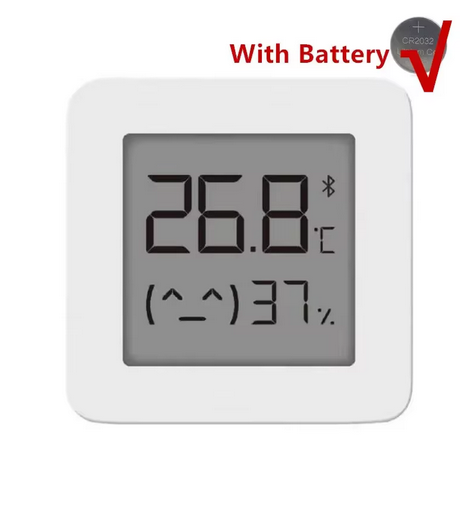
\includegraphics[width=0.4\textwidth]{img/hw_xiaomi_sensor.png}
\caption[Sensor Xiaomi LYWSD03MMC.]{Sensor de temperatura y humedad Xiaomi LYWSD03MMC (Mijia Bluetooth). Se comunica por BLE GATT directo y proporciona lecturas precisas de temperatura, humedad relativa y voltaje de batería sin depender de la nube del fabricante.}
\label{fig:xiaomi_sensor}
\end{figure}

\begin{figure}[h]
\centering
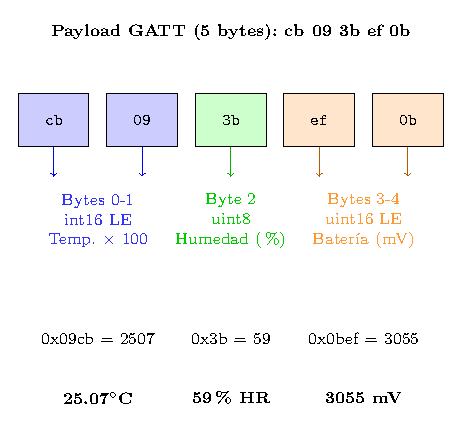
\includegraphics[width=0.75\textwidth]{img/fig_8_5.pdf}
\caption{Decodificación de los 5 bytes de la característica \texttt{ebe0ccc1} del sensor Xiaomi LYWSD03MMC. El payload se lee por GATT sin autenticación.}
\label{fig:ble_decode}
\end{figure}

Una lectura típica \texttt{cb093bef0b} se decodifica como 25.07$^\circ$C, 59\% HR y 3055~mV de batería. El flujo completo (descubrimiento, conexión GATT y desconexión) consume aproximadamente 12~s.

\subsection{Filosofía de Integración y Restricciones}

La integración de cada dispositivo del ecosistema ha seguido dos principios fundamentales:

\begin{itemize}
    \item \textbf{Economía real como factor limitante.} Se descartaron soluciones que habrían acelerado el desarrollo pero requerían inversión adicional (dongle analizador BLE nRF52840, mando universal por infrarrojos), optando por la ingeniería inversa con herramientas ya disponibles. El coste total de las integraciones (sin contar horas de investigación) ha sido de 0~\euro{}.
    \item \textbf{Aprendizaje mediante resolución de problemas reales.} La heterogeneidad de protocolos no es un defecto del ecosistema, sino una característica deliberada. El proyecto demuestra que una capa de orquestación con inteligencia artificial puede unificar dispositivos de distintos fabricantes, protocolos y generaciones (incluso aquellos que no fueron diseñados para interoperar) sin modificar su hardware.
\end{itemize}

\section{Firmware del Nodo ESP32 (\texttt{firmware/})}

El firmware está planificado en C++20 y se estructura en dos responsabilidades:
\begin{itemize}
    \item \textbf{Comunicación con el servidor:} Interfaz serie o TCP/IP para recibir comandos.
    \item \textbf{Comunicación por bus LIN:} Uso del transceptor LINTTL3 para generar y leer tramas del protocolo General/Fujitsu (Series ARHG/ARYG), con regulación de voltaje mediante step-down LM2596.
\end{itemize}

El desarrollo de este firmware no se ha completado dentro del calendario del TFG por dos razones. La primera es de alcance: tras documentar el protocolo LIN del fabricante y analizar el repositorio \texttt{esphome-fujitsu-halcyon} de Omniflux~\cite{omniflux_esphome_fujitsu}, se confirmó que dicho código contiene ya el \textit{parser} de tramas LIN necesario para comunicarse con la máquina General/Fujitsu. Esto reduce drásticamente el trabajo de ingeniería inversa que sería necesario de otro modo, pero su integración con el ecosistema (adaptación del bucle serie, gestión de errores, validación de comandos) sigue siendo una tarea que requiere semanas de desarrollo y pruebas.

La segunda razón es más doméstica que técnica. La máquina de conductos es el único sistema de aire acondicionado de la vivienda, y ponerla fuera de servicio durante el tiempo que durase el desarrollo del firmware (conectando y desconectando el ESP32 del bus LIN, probando comandos, depurando errores) habría dejado a la familia sin refrigeración en pleno mes de junio, cuando las temperaturas en Córdoba superan con facilidad los 38~$^\circ$C. A esta restricción se suma una consideración de planificación: el autor cuenta con experiencia profesional en instalaciones de climatización, lo que le permite evaluar con criterio técnico los riesgos de intervenir el bus LIN de una máquina en producción durante la temporada de máxima demanda. Dado el calendario del TFG, resultó más eficiente dedicar los recursos disponibles a completar las integraciones IoT (Tuya, Xiaomi, FanLamp) y posponer el firmware HVAC como línea de trabajo prioritaria tras la entrega de la memoria.

El hardware necesario está adquirido y cableado (ESP32 DevKit V1, transceptor LINTTL3, regulador LM2596, caja estanca). El ESP32, que actualmente actúa como puente BLE para el ventilador FanLamp, está diseñado para reutilizarse como nodo LIN cuando se aborde esta integración. Queda, por tanto, como la línea de trabajo futura prioritaria.

\section{Integraciones de Hardware}

\subsection{Dispositivos Tuya}
El ecosistema incluye un enchufe inteligente Tuya con medición de consumo, documentado en \texttt{firmware/Enchufe/devices.json}. La integración ha sido completamente validada en la red \textit{air-gapped}.

\subsection{Sensores Xiaomi LYWSD03MMC}
Los sensores de temperatura y humedad se comunican por BLE. Cada sensor está identificado por su dirección MAC y se lee mediante \texttt{ble\_sensors.py}~\cite{bleak}, minimizando el consumo de batería con conexiones puntuales.

\subsection{Ventilador de Techo FanLamp Pro F8808}

El ventilador modelo F8808 de Mikomika, adquirido en AliExpress por 35~\euro{} e instalado personalmente por el autor, representa el dispositivo más complejo del ecosistema en términos de integración. La Figura~\ref{fig:fanlamp} muestra el modelo real instalado en el techo del dormitorio.

\begin{figure}[h]
\centering
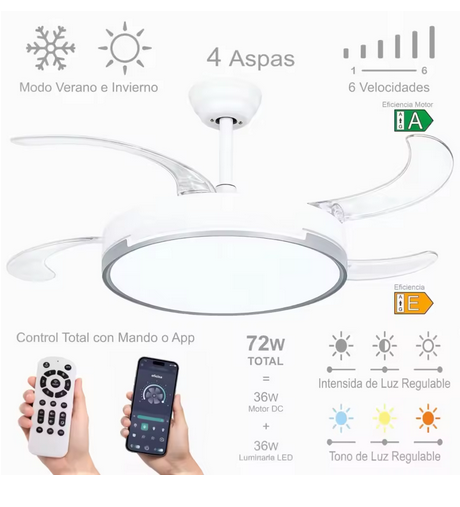
\includegraphics[width=0.4\textwidth]{img/hw_fanlamp.png}
\caption[Ventilador FanLamp F8808 instalado.]{Ventilador de techo FanLamp Pro F8808 de Mikomika, con luz LED regulable (tres temperaturas de color) y cinco velocidades. Su protocolo BLE propietario fue descubierto mediante ingeniería inversa completa durante el proyecto.}
\label{fig:fanlamp}
\end{figure}

\subsubsection{Problema de Integración}
El ventilador no dispone de documentación pública. El fabricante solo ofrece una aplicación móvil propietaria (FanLamp Pro). Cualquier intento de conexión GATT estándar era rechazado tras ~1.5~s. El ventilador exige una autenticación propietaria del protocolo Tencent antes de exponer sus servicios.

\subsubsection{Descubrimiento del Protocolo}
Se decompiló el APK de FanLamp Pro (~60~MB) con \texttt{jadx}. Aunque está desarrollado en Flutter (Dart compilado a ARM64), el análisis reveló que la aplicación \textbf{no utiliza conexiones GATT}, sino \textbf{anuncios BLE} (\textit{BLE Advertisements}). Cada comando se codifica como 13 UUIDs de 16 bits emitidos como datos de servicio.

Al no poder emitir anuncios BLE personalizados desde el portátil por limitaciones de la pila Bluetooth de Linux, se reutilizó el ESP32 DevKit V1 como radio BLE programable, alternando entre modo escáner y modo reproductor.

\subsubsection{Control desde el Ordenador}
Se descubrió que la herramienta \texttt{btmgmt} (paquete \texttt{bluez}) permite emitir anuncios BLE con datos crudos deteniendo temporalmente \texttt{bluetoothd}. El script \texttt{fanlamp\_bt.py} automatiza este proceso. Se han mapeado y verificado 11 comandos:

\begin{table}[h]
\centering
\begin{tabular}{|l|p{6cm}|}
\hline
\textbf{Comando} & \textbf{Efecto} \\
\hline
\texttt{off} & Apaga ventilador y luz \\
\texttt{fan\_on} / \texttt{fan\_off} & Enciende o apaga el ventilador \\
\texttt{light\_on} / \texttt{light\_off} & Enciende o apaga la luz \\
\texttt{1} a \texttt{5} & Velocidad del ventilador (1 = mínima, 5 = máxima) \\
\texttt{night} & Modo noche (luz atenuada) \\
\hline
\end{tabular}
\caption{Comandos disponibles para el ventilador FanLamp F8808.}
\end{table}

\subsubsection{Evolución del Controlador: de BLE directo a Puente ESP32}

El control del ventilador FanLamp ha atravesado dos fases diferenciadas, cada una con sus ventajas y limitaciones. Esta sección documenta la transición del primer prototipo basado en 	exttt{btmgmt} al sistema actual basado en un ESP32 dedicado.

\textbf{Fase 1 --- Control directo por BLE (\texttt{fanlamp\_bt.py}, heredado).} En la primera implementación, los anuncios BLE se emitían directamente desde el adaptador Bluetooth del servidor mediante la herramienta 	exttt{btmgmt} del paquete 	exttt{bluez}. El proceso requería detener temporalmente el demonio 	exttt{bluetoothd}, enviar los anuncios y reactivarlo, todo con permisos de superusuario. Aunque funcional, este enfoque presentaba tres problemas:

\begin{itemize}
    \item \textbf{Monopolización del adaptador Bluetooth:} mientras se controlaba el ventilador, no era posible leer el sensor Xiaomi simultáneamente, ya que ambos usaban la misma radio Bluetooth del PC.
    \item \textbf{Dependencia de 	exttt{sudo}:} cada comando requería ejecución privilegiada para parar y reiniciar 	exttt{bluetoothd}, lo que complicaba la integración con el orquestador.
    \item \textbf{Inestabilidad:} en ocasiones, 	exttt{bluetoothd} no se recuperaba correctamente tras el reinicio, requiriendo intervención manual.
\end{itemize}

La latencia típica de este método era de aproximadamente 3~s por comando.

\textbf{Fase 2 --- Puente ESP32 dedicado (\texttt{fanlamp\_control.py}, actual).} Para resolver las limitaciones de la Fase~1, se incorporó un ESP32 DevKit V1 como radio BLE externa dedicada. El firmware del ESP32 (escrito en C++, disponible en \texttt{firmware/esp32\_fanlamp/src/main.ino}) implementa un bucle que recibe comandos de un solo carácter por puerto serie USB (115200~baud) y emite los pares de anuncios BLE correspondientes (G1~+~G2, 31~bytes cada uno).

El script Python \texttt{fanlamp\_control.py} se comunica con el ESP32 a través del puerto serie, implementando un protocolo de reset DTR para sincronización tras el arranque del microcontrolador y una función \texttt{drain\_until\_ok()} que espera hasta recibir la señal de disponibilidad antes de enviar comandos.

Las ventajas de esta arquitectura son:

\begin{itemize}
    \item \textbf{Radio Bluetooth liberada:} el adaptador del servidor queda libre para la lectura del sensor Xiaomi, permitiendo la operación simultánea de ambos dispositivos.
    \item \textbf{Sin necesidad de 	exttt{sudo}:} la comunicación serie no requiere permisos de superusuario si el usuario pertenece al grupo 	exttt{dialout}.
    \item \textbf{Latencia reducida:} el tiempo de respuesta baja de ~3~s a ~1.5~s por comando, al eliminar la sobrecarga de parar y reiniciar 	exttt{bluetoothd}.
    \item \textbf{Recuperación autónoma:} el ESP32 puede resetearse mediante DTR sin intervención manual, y el script Python detecta y maneja errores de comunicación.
    \item \textbf{HW reutilizable:} el mismo ESP32 que hoy sirve como puente BLE para el ventilador podrá, en el futuro, actuar como puente LIN para la máquina HVAC, evitando la duplicación de hardware.
\end{itemize}

La Tabla~\ref{tab:fanlamp_fases} resume las diferencias entre ambas fases. El flujo de datos actual sigue la ruta: PC (Python) $\rightarrow$ USB serie (carácter) $\rightarrow$ ESP32 (radio BLE) $\rightarrow$ aire (anuncios G1~+~G2) $\rightarrow$ FanLamp. El firmware del ESP32 y el código fuente de \texttt{fanlamp\_control.py} están disponibles en el repositorio del proyecto.

\begin{table}[h]
\centering
\footnotesize
\begin{tabular}{|p{3cm}|p{3.2cm}|p{3.2cm}|}
\hline
\textbf{Aspecto} & \textbf{\texttt{fanlamp\_bt.py} (Fase 1)} & \textbf{\texttt{fanlamp\_control.py} (Fase 2)} \\
\hline
Radio BLE & Adaptador Bluetooth del PC & ESP32 DevKit V1 dedicado \\
Permisos & Requiere \texttt{sudo} & Grupo \texttt{dialout} \\
Convivencia sensor Xiaomi & No (monopoliza BT) & Sí (BT del PC libre) \\
Latencia & $\sim$3~s & $\sim$1.5~s \\
Recuperación ante fallos & Reinicio manual de \texttt{bluetoothd} & Reset DTR automático \\
Reutilización HW & No aplica & Futuro puente LIN HVAC \\
\hline
\end{tabular}
\caption{Comparativa entre las dos fases del controlador del ventilador FanLamp.}
\label{tab:fanlamp_fases}
\end{table}

\section{Estructura del Repositorio}

{\small\begin{verbatim}
luxe-core-ai/
+-- server/                 # Núcleo del sistema (Python)
|   +-- integrations/       # Drivers: Tuya, BLE, HVAC (stub)
|   +-- model_router/       # Enrutador 3 niveles (Tier 0/1/2)
|   |   +-- router.py       #   API HTTP, enrutamiento, prompts
|   |   +-- config.py       #   Patrones zero-inference, escenas
|   |   +-- comfort.py      #   Advisor de confort térmico (ASHRAE 55)
|   |   +-- smart_advisor.py#   Advisor contextual (clima, presencia)
|   +-- sensor_daemon.py    # Daemon de lectura continua (60 s)
|   +-- tools/              # Wrappers CLI invocados por OpenClaw
|   +-- requirements.txt
+-- scripts/                # fanlamp_bt.py, fanlamp_control.py
+-- firmware/               # Código para microcontroladores
|   +-- esp32_fanlamp/      #   Puente BLE para FanLamp y sensores
+-- tests/                  # Suite de integración automatizada
|   +-- test_integration.py
+-- docs/                   # Memoria del TFG (LaTeX)
|   +-- sections/           #   Capítulos de la memoria
|   +-- appendices/         #   Anexos (usuario, código, glosario)
|   +-- figures/            #   Código fuente de figuras TikZ
|   +-- img/                #   Imágenes y capturas
|   +-- design_decisions/   #   Registros de decisión (ADR)
|   +-- compile_docs.sh     #   Script de compilación
|   +-- references.bib      #   Base de datos bibliográfica
+-- meta/                   # Roadmap, estado del proyecto
\end{verbatim}}

\noindent El directorio \texttt{server/} contiene el núcleo del sistema: los \textit{drivers} de dispositivos (Tuya~\cite{tinytuya}, BLE~\cite{bleak}), el enrutador inteligente de tres niveles (Model Router v2), el daemon de sensorización continua y los \textit{wrappers} CLI invocados por OpenClaw. El módulo \texttt{model\_router/} alberga la lógica central de enrutamiento, los patrones \textit{zero-inference}, los asesores de confort térmico~\cite{ashrae55_2023, rothfusz_1990} y contexto exterior, y los \textit{prompts} del clasificador 1.5B. El directorio \texttt{scripts/} contiene los scripts de control del ventilador FanLamp. En \texttt{firmware/} se encuentra el código del ESP32 para el puente BLE. La carpeta \texttt{tests/} incluye la suite de pruebas automatizadas. En \texttt{docs/} se encuentra la presente memoria en \LaTeX{}, las figuras editables en TikZ y los registros de decisión (ADR).

En el capítulo siguiente se presentan los resultados de validación de cada uno de los módulos descritos, verificados sobre el hardware real del proyecto en la red \textit{air-gapped}.
